\documentclass{article}
%% Chapter 1 Section 10: Exponentiation

\usepackage{amsmath}
\usepackage{palatino}
\usepackage{tikz}

\newcommand{\curry}[1]{\emph{curry}(#1)}
\newcommand{\eval}{\emph{eval}}
\newcommand{\id}{\emph{id}}
\newcommand{\cset}{\mathbf{Set}}
\newcommand{\cseta}{\mathbf{Set}^{\rightarrow}}
\newcommand{\csetset}{\cset \times \cset}
\newcommand{\fpl}{\mathbf{FPL}}
\newcommand{\powset}{\mathcal{P}}
\newcommand{\set}[1]{\{#1\}}

\begin{document}

\begin{enumerate}
\item [1.10.5.1]
  %% TODO
  An example of a small, finite category with binary products and a terminal object but no exponentials is \ldots

  Surprisingly hard to find.
  It must be hiding in plain sight.

\item [1.10.5.2]
  Exponentation in $\csetset$ is componentwise.
  That is, every pair of $\csetset$ objects determines an exponential.
  
  Let $A \times B$ and $C \times D$ be two objects in $\csetset$.
  The exponential of this pair is an object $C^A \times D^B$.
  The function $\eval$  has domain $(C^A \times D^B) \times (A \times B)$ and codomain $C \times D$.
  Application is componentwise.
  The result of $\eval((f, g), (a,b))$ is the pair $(f a, g b)$.

  Then for every arrow $g : E \times (A \times B) \rightarrow C \times D$, we have a unique arrow $\curry{g}$ that maps the $\csetset$ object $E$ to the exponential $C^A \times D^B$.
  This arrow is uniquely determined comoponentwise; because $E$ is itself a pair of $\cset$ objects, each with an exponential, we obtain the $csetset$ object by taking the exponential of the first and second member of the pair.
  
  The entire construction is summarized in the below diagram.
  Parenthesis are inserted for readability.
  \begin{center}
    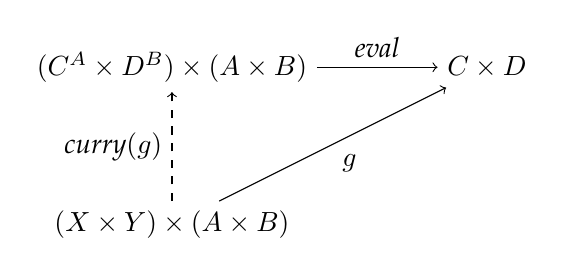
\begin{tikzpicture}
      \node (1) {$(C^A \times D^B) \times (A \times B)$};
      \node[below of=1, yshift=-1cm] (2) {$(X \times Y) \times (A \times B)$};
      \node[right of=1,xshift=3cm] (3) {$C \times D$};
      
      \draw[->] (1) -- node[above] {$\eval$} (3);
      \draw[->] (2) -- node[below right] {$g$} (3);
      \draw[->,dashed] (2) -- node[left] {$\curry{g}$} (1);
    \end{tikzpicture}
  \end{center}

\newpage
\item [1.10.5.3]
  An exponential object in $\cseta$ is a collection of arrows between two $\cseta$ objects.

  An object in $\cseta$ is an arrow $f: A \rightarrow B$ between two sets.
  An arrow between objects $f : A \rightarrow B$ and $f' : A' \rightarrow B'$ in $\cseta$ is a pair of arrows $(a,b)$ where $a : A \rightarrow A'$ and $b: B \rightarrow B'$ are such that $f' \circ a = b \circ f$.
  \begin{center}
    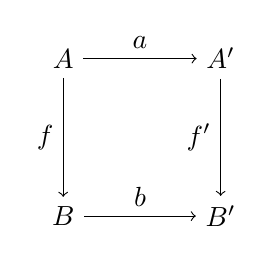
\begin{tikzpicture}
      \node (1) {$A$};
      \node[right of=1,xshift=1cm] (2) {$A'$};
      \node[below of=1,yshift=-1cm] (3) {$B$};
      \node[right of=3,xshift=1cm] (4) {$B'$};
      
      \draw[->] (1) -- node[above] {$a$} (2);
      \draw[->] (1) -- node[left] {$f$} (3);
      \draw[->] (2) -- node[left] {$f'$} (4);
      \draw[->] (3) -- node[above] {$b$} (4);
    \end{tikzpicture}
  \end{center}

  Hence an exponential object $f'^f$ is the collection of all such $\cseta$ arrows $(a,b)$.
  Filling in the canonical diagram for exponentials, we have the following, where $f'' : A'' \rightarrow B''$ is any other object in $\cseta$.
  \begin{center}
    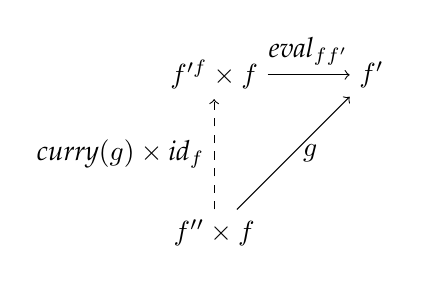
\begin{tikzpicture}
      \node (1) {$f'^f \times f$};
      \node [below of=1,yshift=-1cm] (2) {$f'' \times f$};
      \node [right of=1,xshift=1cm] (3) {$f'$};
      
      \draw[->] (2) -- node [right] {$g$} (3);
      \draw[->,dashed] (2) -- node [left] {$\curry{g} \times \id_f$} (1);
      \draw[->] (1) -- node [above] {$\eval_{ff'}$} (3);
    \end{tikzpicture}
  \end{center}
  Here $\curry{g}$ is the uniquely determined function that brings a $\cseta$ object $f''$ to one of the arrows $f \rightarrow f'$ in the exponential $f'^f$.

\newpage
\item [1.10.5.4]
  To show that $\curry{\eval_{AB}} = \id_{(B^A)}$, we first consider what we know about $\eval_{AB} : B^A \rightarrow B$.
  \begin{center}
    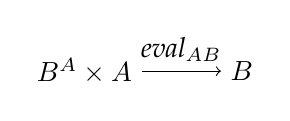
\begin{tikzpicture}
      \node (1) {$B^A \times A$};
      \node [right of=1,xshift=1cm] (3) {$B$};
      
      \draw[->] (1) -- node [above] {$\eval_{AB}$} (3);
    \end{tikzpicture}
  \end{center}
  
  Assuming $B^A$ is an exponential object and that $\eval_{AB}$ is the arrow associated with this exponential, we know that for any other object $C$ and arrow $g : C \times A \rightarrow B$ we have a unique mediating arrow $\curry{g} : C \rightarrow B^A$ such that the following diagram commutes.
  \begin{center}
    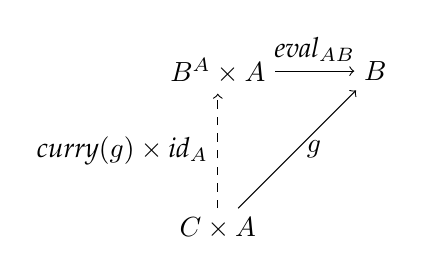
\begin{tikzpicture}
      \node (1) {$B^A \times A$};
      \node [below of=1,yshift=-1cm] (2) {$C \times A$};
      \node [right of=1,xshift=1cm] (3) {$B$};
      
      \draw[->] (2) -- node [right] {$g$} (3);
      \draw[->,dashed] (2) -- node [left] {$\curry{g} \times \id_A$} (1);
      \draw[->] (1) -- node [above] {$\eval_{AB}$} (3);
    \end{tikzpicture}
  \end{center}

  One such possible $g$ is $\eval_{AB}$.
  It takes an object $C = B^A$ to $B$.
  Therefore, there must be a unique arrow $\curry{\eval_{AB}} : B^A \rightarrow B^A$ that makes the diagram commute.
  \begin{center}
    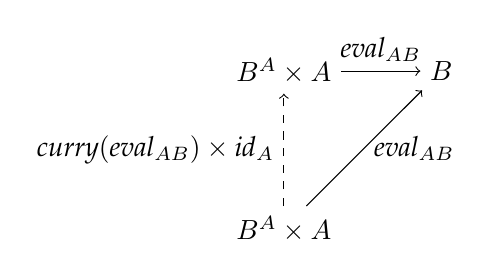
\begin{tikzpicture}
      \node (1) {$B^A \times A$};
      \node [below of=1,yshift=-1cm] (2) {$B^A \times A$};
      \node [right of=1,xshift=1cm] (3) {$B$};
      
      \draw[->] (2) -- node [right] {$\eval_{AB}$} (3);
      \draw[->,dashed] (2) -- node [left] {$\curry{\eval_{AB}} \times \id_A$} (1);
      \draw[->] (1) -- node [above] {$\eval_{AB}$} (3);
    \end{tikzpicture}
  \end{center}
  
  However, $\id_{B^A}$ is another unique arrow that also makes this diagram commute.
  This is more clearly shown if we collapse identical nodes in the diagram.
  \begin{center}
    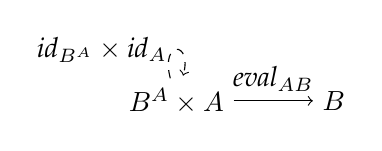
\begin{tikzpicture}
      \node (1) {$B^A \times A$};
      \node [right of=1,xshift=1cm] (3) {$B$};
      
      \draw[->,dashed] (1) edge [loop above] node [left] {$\id_{B^A} \times \id_A$} (1);
      \draw[->] (1) -- node [above] {$\eval_{AB}$} (3);
    \end{tikzpicture}
  \end{center}

  Therefore $\curry{\eval_{AB}} = \id_{B^A}$.

\newpage
\item [1.10.5.5]
  The goal is to show that $(B^A)^{A'}$ is isomorphic to $B^{A \times A'}$ in any cartesian-closed category.

  One direction of this argument is fairly straightforward.
  The exponential $B^{A \times A'}$ defines a function $\eval_1 : B^{A \times A'} \times (A \times A') \rightarrow B$, which in turn uniquely determines a function $\curry{g}$ for any function $g : C \times (A \times A') \rightarrow B$.
  Taking $C$ to be $(B^A)^{A'}$, we can define $g : (B^A)^{A'} \rightarrow (A \times A') \rightarrow B$ as $\mathbf{fun}~f~(a,a') = f~a'~a$.
  \begin{center}
    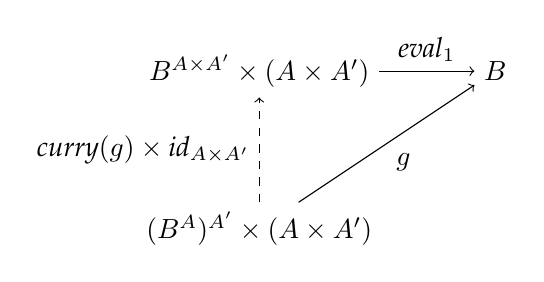
\begin{tikzpicture}
      \node (1) {$B^{A \times A'} \times (A \times A')$};
      \node [below of=1,yshift=-1cm] (2) {$(B^A)^{A'} \times (A \times A')$};
      \node [right of=1,xshift=2cm] (3) {$B$};
      
      \draw[->] (2) -- node [below right] {$g$} (3);
      \draw[->,dashed] (2) -- node [left] {$\curry{g} \times \id_{A \times A'}$} (1);
      \draw[->] (1) -- node [above] {$\eval_1$} (3);
    \end{tikzpicture}
  \end{center}
  Now the uniquely determined arrow $\curry{g} : (B^A)^{A'} \rightarrow B^{A \times A'}$ is half our isomorphism.

  For the reverse, we need to unroll the definition of $(B^A)^{A'}$.
  As is, it defines an evaluation function that accepts one function $f : A' \rightarrow A$ to return a $B$.
  Rather than taking a function on objects, we want to take just objects.

  Let $\eval_2 : (B^A)^{A'} \times A' \rightarrow B^A$ and $\eval_3 : B^A \times A \rightarrow B$ in the obvious way.
  Then with a slight abuse of notation we can use their composition to obtain a $B$ from a pair $A' \times A$.
  This composition $\eval_3 \circ \eval_2$ then uniquely determines a function $\curry{g'} : C \rightarrow B^{A \times A'}$ for each function $g' : C \times (A' \times A) \rightarrow B$.
  Let $C$ be $B^{A \times A'}$ and let $g'$ permute its arguments then apply $\eval_1$ from above.
  Now $\curry{g'}$ is the unique arrow taking $B^{A \times A'}$ to $(B^A)^{A'}$, thus completing the isomorphism.
  \begin{center}
    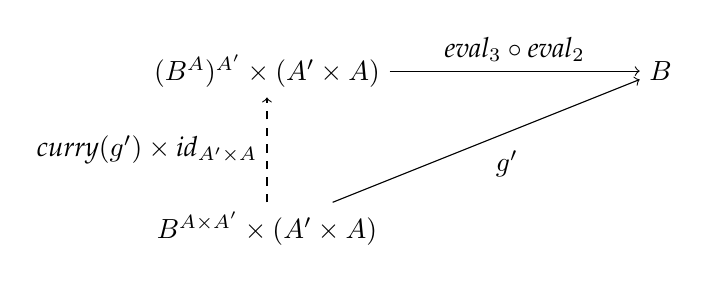
\begin{tikzpicture}
      \node (1) {$(B^A)^{A'} \times (A' \times A)$};
      \node [below of=1,yshift=-1cm] (2) {$B^{A \times A'} \times (A' \times A)$};
      \node [right of=1,xshift=4cm] (3) {$B$};
      
      \draw[->] (2) -- node [below right] {$g'$} (3);
      \draw[->,dashed] (2) -- node [left] {$\curry{g'} \times \id_{A' \times A}$} (1);
      \draw[->] (1) -- node [above] {$\eval_3 \circ \eval_2$} (3);
    \end{tikzpicture}
  \end{center}

\newpage  
\item [1.10.5.6]
  We show the category defined by the powerset of a set $S$ and the subset relation $\subseteq$ is cartesian closed by showing it has binary products and exponentials.

  The binary product of two elements $A,B$ of the powerset $\powset(S)$ is the intersection of the elements.
  This ensures that the product object is a subset of both $A$ and of $B$.
  Moreover, it induces a unique arrow from any other object $X$ that is a subset of both $A$ and $B$ because $A \cap B$ is the largest subset of both.

  Two examples are below.
  One has an empty intersection and the other a non-empty intersection.
  \begin{center}
    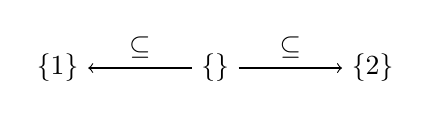
\begin{tikzpicture}
      \node (1) {$\set{}$};
      \node [left of=1,xshift=-1cm] (2) {$\set{1}$};
      \node [right of=1,xshift=1cm] (3) {$\set{2}$};
      
      \draw[->] (1) -- node[above] {$\subseteq$} (2);
      \draw[->] (1) -- node[above] {$\subseteq$} (3);
    \end{tikzpicture}
    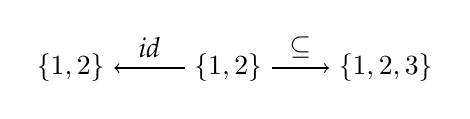
\begin{tikzpicture}
      \node (1) {$\set{1,2}$};
      \node [left of=1,xshift=-1cm] (2) {$\set{1,2}$};
      \node [right of=1,xshift=1cm] (3) {$\set{1,2,3}$};
      
      \draw[->] (1) -- node[above] {$\id$} (2);
      \draw[->] (1) -- node[above] {$\subseteq$} (3);
    \end{tikzpicture}
  \end{center}

  The exponent of two elements $A,B$ of $\powset{S}$ can be encoded as $B$ if $B \subseteq A$, otherwise it must be $S$.
  I suspect there is a cleaner way to convey this, but the obvious formula $\neg A \cup B$ and similar variants fail.
  
  If $B \subseteq A$, then $B^A \subseteq B$ must hold.
  We choose $B^A = B$ because it is the largest set for which the equality is true.
  This, combined with the fact that our category is thin, gives $B^A$ the desired universal property.
  
  However if $A \subseteq B$, then for any object $C$, the unique arrow $f : A \rightarrow B$ composed with $\pi_2$ gives a map from the product $C \times A$ to $B$.
  Therefore $C$ can be any object in the set and therefore $B$ must be the set $S$ for the universal property to hold.

\vfill{}
\item [1.10.5.7]
  If we consider $S$, the set of sentences of propositional logic, as a preorder $(S, \le)$ where $p \le q$ means ``from $p$ we can derive $q$'', then we can show that the preorder forms a cartesian closed category.
  Objects are elements of $S$; that is, sentences of propositional logic.
  An arrow between two objects $p$ and $q$ exists if and only if $p \le q$.
  Composition then follows by transitivity of $\le$ and identity arrows follow from the reflexivity of $\le$.

  Pierce defines the binary product $p \times q$ as the conjunction $p \wedge q$, which makes sense because given $p \wedge q$ we can derive either $p$ or $q$.
  Likewise for a product object we can extract either $p$ or $q$ using the right projection arrow.
  The universality property is satisfied by observing that if sentence $x$ lets us derive both $p$ and $q$ then it will allow us to derive $p \wedge q$ in propositional logic.
  Therefore $x \le p \wedge q$ and we have the desired arrow from $x$ to $p \times q$.

  For exponents, Pierce claims the sentence ``$p$ implies $q$'' should correspond to the object $q^p$.
  To validate this claim, we first observe that $\eval$ corresponds to \emph{modus ponens}.
  Hence $q^p \wedge p \le q$ and we have an arrow from $q^p \times p \rightarrow q$.
  Then supposing there existed an arrow $g : r \times p \rightarrow q$ we could derive a unique arrow $\curry{g} : r \rightarrow q^p$.
  In terms of propositional logic, assuming we have $p$ the weakest precondition for deriving $q$ is ``$q$ implies $p$''.
  Therefore any other proposition $r$ that we can replace for $q^p$ and still derive the same conclusion must itself imply $q^p$.
  This implies that $r \le q$, thus yielding our curry arrow.
  
\vfill{}
\item [1.10.5.8]
  We can extend $\fpl$ with higher-order functions by adding exponentials.
  This would make it possible to reason about all functions of a certain type, say $\emph{bool} \rightarrow \emph{int}$ in the domain or codomain of an arrow.
  
\vfill{}
\end{enumerate}

\end{document}
